\section{Test Setup}\label{sec:test_setup}
In order to perform tests for these criteria, we need to have a setup to do so.

Testing the offset between two audio sources is a signal processing
task. To make the signal processing easy and effective, a clear signal is
needed. Additionally the signal needs to be synchronized between the
channels at recording time, since otherwise the analysis would be
mislead by desync in the recording. Luckily most computers include
a port for doing just that, a stereo microphone port.

The stereo microphone port in the test computer is a \ac{TRS} jack
connector, with a common ground between the two channels. To separate
the channels into separate mono tracks we used a \ac{TRS} to \ac{RCA}
splitter, and a custom \ac{RCA} to mono \ac{TS}, to capture one of the two
channels from the audio sources.
An illustration of the test setup together with the jack cable can be seen on \cref{fig:test_setup}.

\begin{figure}[!bht]
    \centering
    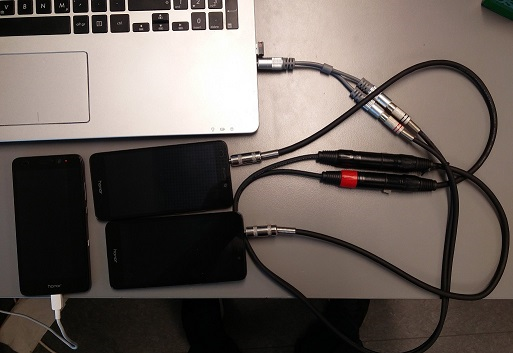
\includegraphics[width=0.8\textwidth]{img/test_setup.png}
    \caption{An illustration of the test setup with the three phones and the jack cable.}
    \label{fig:test_setup}
\end{figure}

% Troels additions below
Furthermore we limit our tests to a Master/Slave/Slave setup, that is;
one phone acts as a master, and we perform the tests on two slaves
connected to it. This makes the two devices under test as similar as
possible, since neither has the reference sound.
Ideally we would also record the reference, the Master, but since we only have two input channels that is not possible.

In the tests we use three Android phones:
\begin{dankscription}{\bfseries}{Master}
	\item[Master]OnePlus One (Android 6.0.1, Kernel 3.4.112-cyanogenmod-g62d75e8)
	\item[Slave 1]Moto X Style (Android 6.0.1, Kernel 3.10.84-perf-gb67345b)
	\item[Slave 2]OnePlus Two (Android 6.0.1, Kernel 3.10.84-perf+)
\end{dankscription}

\subsection{Test Scripts}
We automate the mechanical part of the testing, such as doing the
analysis and controlling the variables. To do so we use scripts written
in Python, which use the \ac{ADB} interface to control the Android
phones. The tests are executed by a Python script to ensure
consistency and minimize the chances of error caused by humans.

Measuring the offset between the two signals is a signal processing
task. Within the field of signal processing, the specific measure is
called cross correlation. 

To illustrate the principle of using cross correlation to measure the offset between two identical signals, we made \cref{fig:cross_cor}.
In it the blue line $g$, and the purple line $f$, are two identical signals, but they are offset in time, which is the $x$-axis.
Finding the offset can be done by shifting one of them in time, while maximizing the area of their intersection, depicted as $g \star f$.
The shift where the area of the intersection is maximum, is the offset of the two signals.

Cross correlation is normally
a computationally intensive task, but due to the Convolution
Theorem\cite{conv_theo}, it can be solved rather quickly with \ac{FFT}.
The algorithm to calculate the \ac{FFT} of the audio offset thus becomes
doing a \ac{FFT} on one of the signals, and multiplying the results with
a time reversed \ac{FFT} of the other. Finally we do an inverse \ac{FFT}
to get the actual correlation value. The index of the maximum value is
the sample offset which gives the best correlation.
By multiplying the
number of samples by the time between samples, we calculate the
millisecond offset between the two audio tracks.



%optimere a * b, cross corrolation, lave figur med overlap
%forskyder over tid. 

\subimport{}{cross_cor_fig}

The scripts used for testing can be seen in \cnameref{magicscripts}.

To determine the accuracy and reliability of the tests, we do what we
call an assurance test. The variable we need to assure
ourselves of, is inter-stereo delay of the microphone input on the
measurement computer. If there is an intrinsic delay between the left and
right channel of the computer, the whole test will be
compromised, or at least in need of adjustment. We use the delay
measuring script above, along with a standard AUX cable,
and the test song in mono, to detect the delay
between the left and right channel. In our equipment the delay is 0 ms
consistently, which means the results wont be tainted by inter-stereo
delay.

\subsection{Test sample}
We use the song \textit{Goodness Gracious} by \textit{Ellie Goulding}.  We did not
want the apps to change song, possibly causing a resync, while testing.
To avoid that possibility we loop the song for 2 hours within
a single mp3 file.

\subsection{Connecting}
Since the apps being tested are network connected systems, we have to
connect them before the test can begin. The connection procedure is
slightly different for each app. Common for both apps is that we use
three devices to test, one is the ``master'' while the others are
``slaves''. The ``slaves'' are the ones connected to the computer
with the dual mono to stereo cable described earlier, and where we are
measuring the offset.

\paragraph{AmpMe}
AmpMe allows the devices to connect over the public Internet. We test
them on the AAU internal network, where they are technically connected,
but the internal network topology makes them unable to connect directly.
To connect slaves with the master, we start the master playing a song,
thereby starting a ``party'' and allowing the slave devices to
connect. Once the slaves have connected we restart the song on the
master and wait for the app to resume playback.

\paragraph{SoundSeeder}
SoundSeeder does require the devices to be able to connect directly. We
fulfilled that requirement by having the master serve a ad-hoc hotspot,
which allowed the devices to connect, while keeping the slaves
similarly configured. SoundSeeder does not require a song to be playing
for it to connect. For the tests we connect the slaves to the master,
and only after they are connected begin playback.

\subsection{Volume}
The volume of the devices should not be particularly important, since
the method we use for correlation should not care about the relative
amplitude. Regardless we will need to keep the volume low to avoid
clipping, since the microphone input is amplified. For the tests we keep
the volume levels of both devices at 3 steps above the minimum in
Android.

